\documentclass[class=book, crop=false]{standalone}
\usepackage[subpreambles=true]{standalone}
\usepackage{import}
\usepackage[utf8]{inputenc}
\usepackage[margin=1.2in]{geometry}
\usepackage[sorting = none,
            doi = true  %lesedato for url-adresse
            ]{biblatex} %none gir bibliografi i sitert rekkefølge
\addbibresource{reference.bib}
\usepackage{csquotes}
\usepackage{pgfplotstable}
\usepackage{booktabs}
\usepackage{pdflscape}
\usepackage{afterpage}
\usepackage{capt-of}% or use the larger `caption` package
\pgfplotsset{compat=1.15}

\begin{document}
\section{Programming software}
Python is the programming language used for this solving this task. Python is an open-source software that has several packages for machine learning and power flow calculations \cite{python_web}. In this thesis, \textit{pandapower} is the python package used for defining an electric power system and preforming power flow calculations\cite{pandapower}. \textit{Keras} is the Python package used for training a reinforcement agent \cite{keras_chollet2015}.

\section{Pandapower}
Pandapower is a time independent simulation tool, which means that it finds steady state solutions to a power flow problem. Consequently, the transitions from one state to another is not covered in this thesis.

This section will describe the different electrical elements available in pandapower and how they are physically modelled.
\subsection{Lines}
Table \ref{tab:standard_lines_pandapower} shows the available standard line that can be chosen with corresponding parameter values. Custom parameters can also be specified using the method \texttt{pandapower.create\_line\_from\_parameters}
\begin{table}[]
    \centering
    \pgfplotstabletypeset[
col sep = comma,
string type,
every head row/.style={before row=\toprule,after row=\midrule},
every last row/.style={after row=\bottomrule},
display columns/0/.style={string type,column name={}}
]
{data/linetypes.csv}
    \caption{Standard lines available in pandapowers with values for resistance \textit{r}, inductance \textit{x}, capacitance \textit{c}, max current \textit{I} and cross sectional area \textit{Q} and line type. “ol” is overhead line and “cs” is underground cable system}
    \label{tab:standard_lines_pandapower}
\end{table}
The line are modelled using the $\pi$-equivalent model, mentioned in section \ref{section:pi_model}.

\subsection{Generators}
Pandapower has two generator types. The first type is simply called generator and is modelled as a PV-bus. In other words, the active power production $P$ and voltage magnitude $|U|$ is are known when solving the power flow equations. Generators can be created using the method \texttt{pandapower.create\_gen}, where nominal values for apparent power and voltage can be specified. The second type is the static generator, where the active power $P$ and reactive power $Q$ is specified (PQ-bus). Static generators are created using \texttt{pandapower.create\_sgen}. Pandapower models power from the consumer perspective, so negative values for active power $P$ corresponds to generation of power.

\subsection{Loads}
The load in pandapower is modelled as a PQ-bus, where active and reactive power are known. Loads are created using the method \texttt{pandapower.create\_load}. The loads can also be modelled with constant impedance $Z$, current $I$ and $P$. In other words, replacing reactive power with current and impedance.

\subsection{Transformers}
Pandapower offers both two-winding and three-winding transformers that can be created from standard types using the \texttt{pandapower.create\_transformer} method, or from parameters using the method
\texttt{pandapower.create\_transformer\_from\_parameters}. The transformers can be modelled as a $\pi$-transformer or a $t$-transformer. The transformers can have settings for tap-position and phase-shifting of the voltage, which are a possible control variables for a reinforcement agent.  

\subsection{Storage}
It is possible to connect a storage element to a power grid using the \texttt{pandapower.create_storage} method. The storage element is modelled as a PQ-node. Because simulations in pandapower is time-independent and only find steady state solution, it does not update the capacity of a storage during power flow calculations. Available energy in the storage element must therefore be updated manually according to some predefined timescale when several power flow calculations are performed.  


\section{Data structures in pandapower}

Pandapower stores information about components in a net in pandas DataFrames, which make it easy to inspect the output of a power flow calculation. Figure \ref{fig:method:loading_example_net} shows a case net and the components included in it. 

\begin{figure}[H]
    \center
    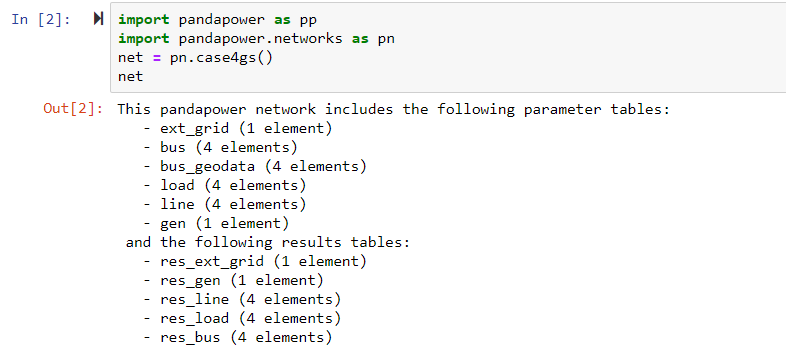
\includegraphics[height=6cm, width=12cm]{figures/case4g_show_net.PNG}
    \caption[size = 9]{Loading an example net in pandapower}
    \label{fig:method:loading_example_net}
\end{figure}
Each of the elements listed have a corresponding pandas DataFrame. The elements without "res" at the beginning are parameter tables and have information about nominal and max/min values for the components. Figure \ref{fig:method:line_bus_dataframe} shows the parameter table for the line and bus.

\begin{figure}[H]
    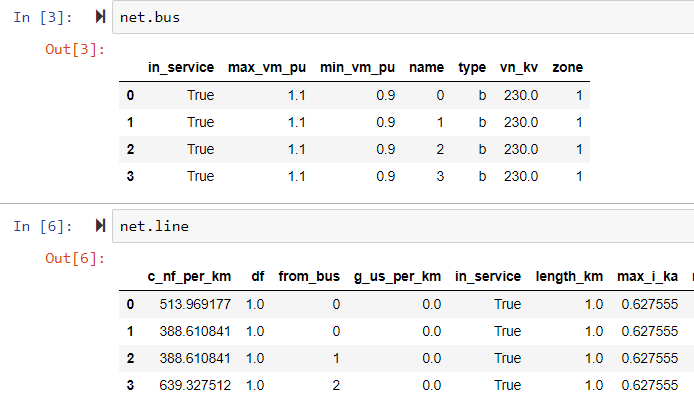
\includegraphics[height=7cm, width=13.5cm]{figures/case4g_line_bus.PNG}
    \caption[size = 9]{Parameter table in pandapower. There are more columns in net.line}
    \label{fig:method:line_bus_dataframe}
\end{figure}
All of the components will have a result table after the power flow calculation is performed, using the method \texttt{pandapower.runpp}. Figure \ref{fig:method:res_line_bus_dataframe} shows the result table for the bus and line.

\begin{figure}[H]
    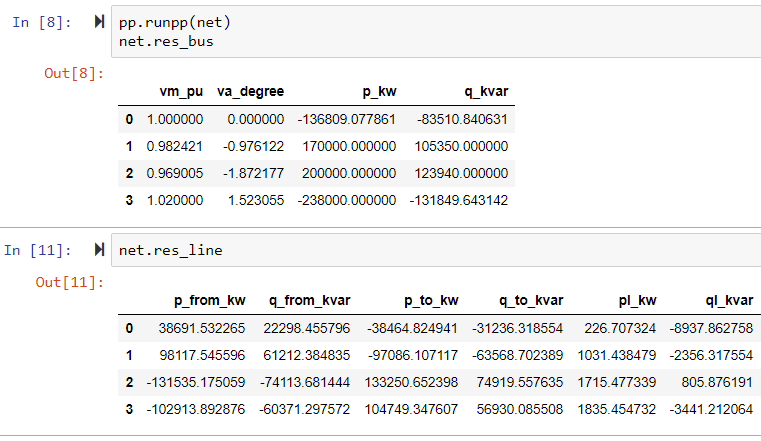
\includegraphics[height=8cm, width=14cm]{figures/case4g_line_bus_res.PNG}
    \caption[size = 9]{Result table in pandapower. There are more columns in net.res\_line}
    \label{fig:method:res_line_bus_dataframe}
\end{figure}















\end{document}

